% ---------
%  Compile with "pdflatex hw0".
% --------
%!TEX TS-program = pdflatex
%!TEX encoding = UTF-8 Unicode

\documentclass[11pt]{article}
\usepackage{amsmath}
\usepackage{amssymb}
\usepackage{jeffe,handout,graphicx}
\usepackage[utf8]{inputenc}		% Allow some non-ASCII Unicode in source

% =========================================================
%   Define common stuff for solution headers
% =========================================================
\pagenumbering{arabic}
\Class{ECE 498 ICC}
\Semester{Spring 2020}
\Authors{1}
\AuthorOne{Jin Yucheng}{yucheng9}
%\AuthorTwo{Friday Caliban}{fcaliban}
%\AuthorThree{Duncan Quagmire}{dquagmir}
%\Section{}

% =========================================================
\begin{document}

% ---------------------------------------------------------


\HomeworkHeader{3}{1}	% homework number, problem number

\begin{solution}
(1) Consider an IoT architecture for a \textbf{smart healthcare system}: \footnote{Luca Catarinucci, et al. "An IoT-Aware Architecture for Smart Healthcare Systems". \textit{IEEE INTERNET OF THINGS JOURNAL}, Vol. 2, No. 6. Dec. 2015}
\begin{itemize}
\item \textbf{Purpose}: A smart healthcare system that could monitor and keep track of a patient's health condition, especially, when it detects an emergency (for example, a heart attack), the system will immediately send alert to the hospital/nursing home.
\item \textbf{Behavior}: Have auto and manual modes. In auto mode, the system will automatically collect and process the patient's biomedical data on a fixed time interval. In manual mode, the 
system provides the option of manually update data. Both modes will send an emergency alert if necessary.
\item \textbf{Data Analytics Requirement}: This system should perform local analysis of the biomedical data collected, since the accuracy of data is one of the top concerns, so this system requires robust sensors.
\item \textbf{Security Requirement}: This system should have basic user authentication capability, such that only the patient himself/herself, hospital/nursing home, and patient's family members can have access to the biomedical data collected.
\end{itemize}
(2) For this problem,
\begin{center}
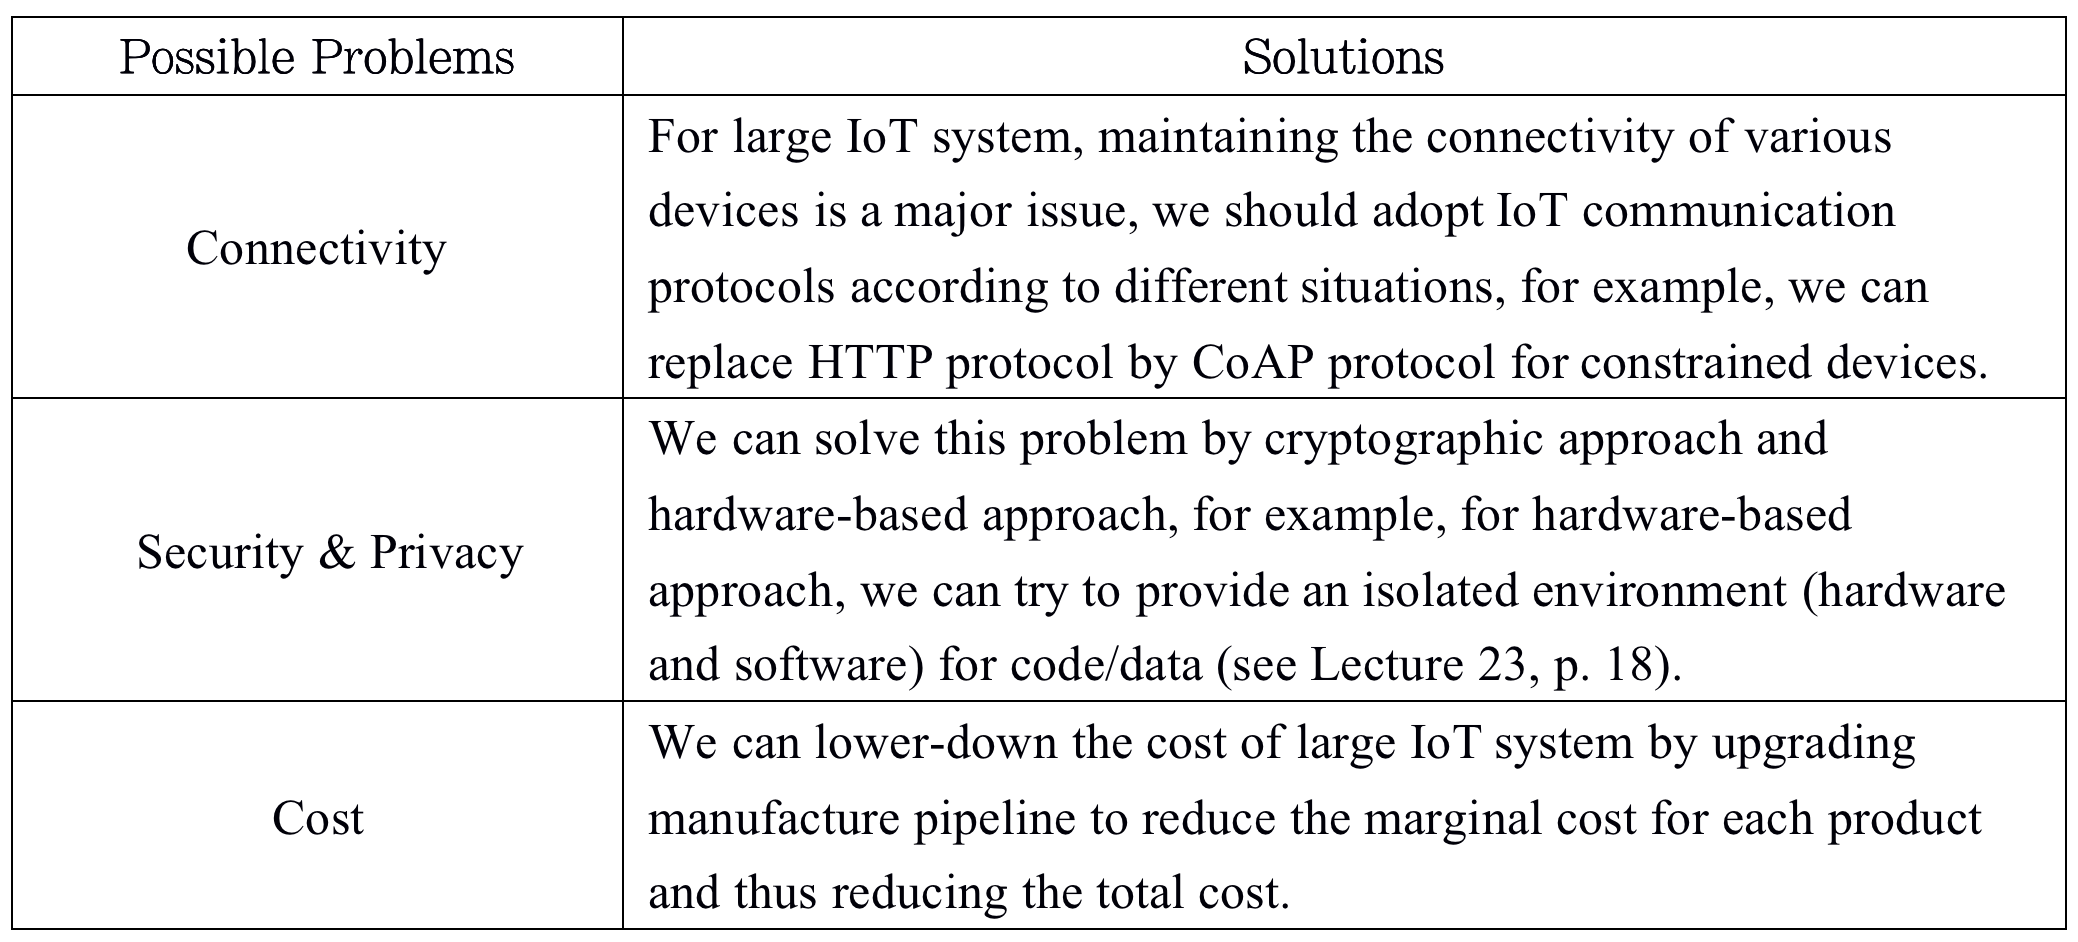
\includegraphics[width=15cm]{p1.png}
\end{center}
(3) According to the conditions,
\begin{itemize}
\item For each
active user under the household,
\begin{itemize} 
\item They must share the same home address.
\item But with distinct age, payment method and billing history.
\end{itemize}
\pagebreak
\item For each vehicle
registered, 
\begin{itemize} 
\item We need the following information: license plate number, plate
sticker valid through, garage address, manufacturer, vehicle type and number
of axis. 
\item Each vehicle needs to be registered under exactly one valid user.
\end{itemize} 
\end{itemize}
I've came up with my idea,
\begin{center}
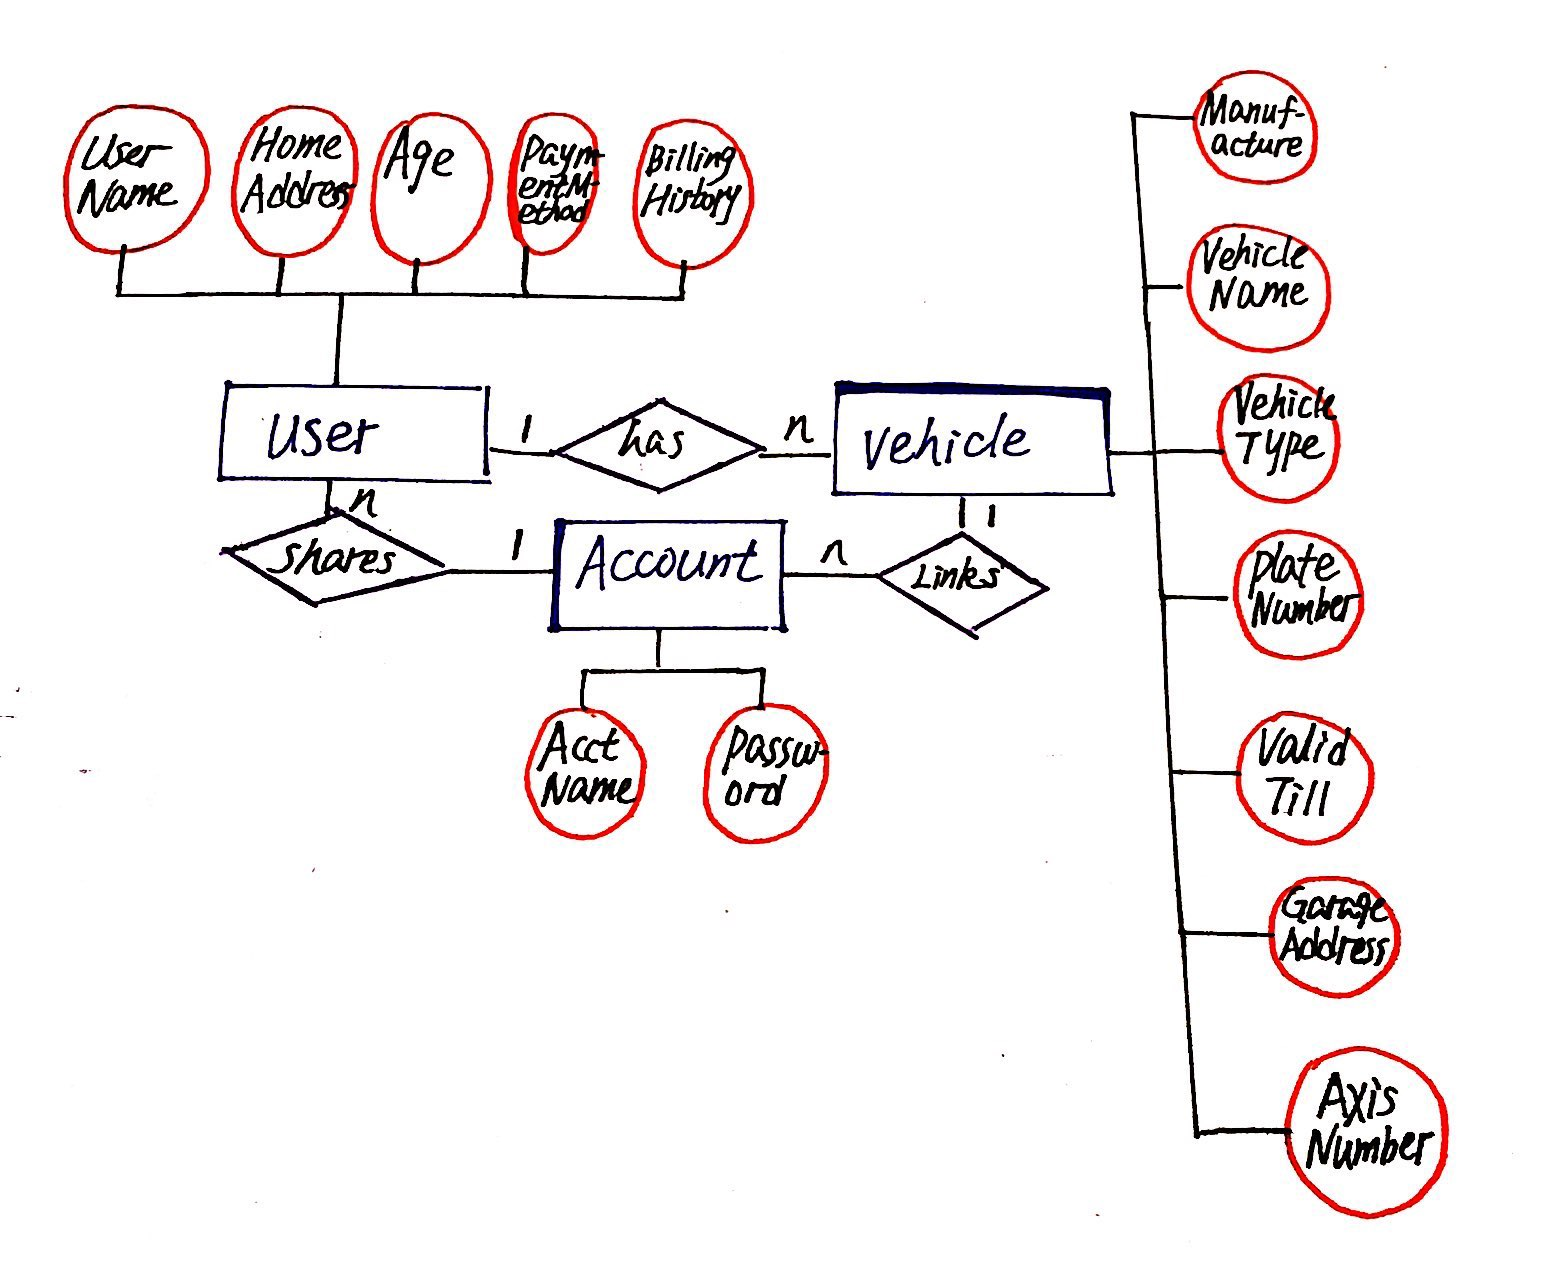
\includegraphics[width=15cm]{p1_2.jpg}
\end{center}
(4) There are many databases that are provided by Amazon AWS, such as Amazon Aurora, Amazon RDS, and Amazon Redshift. The database should store the information of the users and their vehicles, they are calculated as,
\begin{itemize} 
\item Overhead Data: $2,706,000 \times 16$ = $43,296,000$ KB
\item User Data: $2,706,000 \times 3.2 \times 64$ = $554,188,800$ KB
\item Vehicle Data: $2,706,000 \times 2.1 \times 128$ = $727,372,800$ KB
\end{itemize} 
The total data is $\frac{43,296,000 + 554,188,800 + 727,372,800}{1024 \times 1024}$ = $1263.5$ GB.
\\
\\
Since the daily traffic is $1,575,670$, for $30$ days in a month, there are $1,575,670 \times 30$ = $47.27$ million requests. 
\\ 
\\
According to the pricing information\footnote{https://aws.amazon.com/rds/aurora/pricing/?nc=sn\&loc=4},
\begin{center}
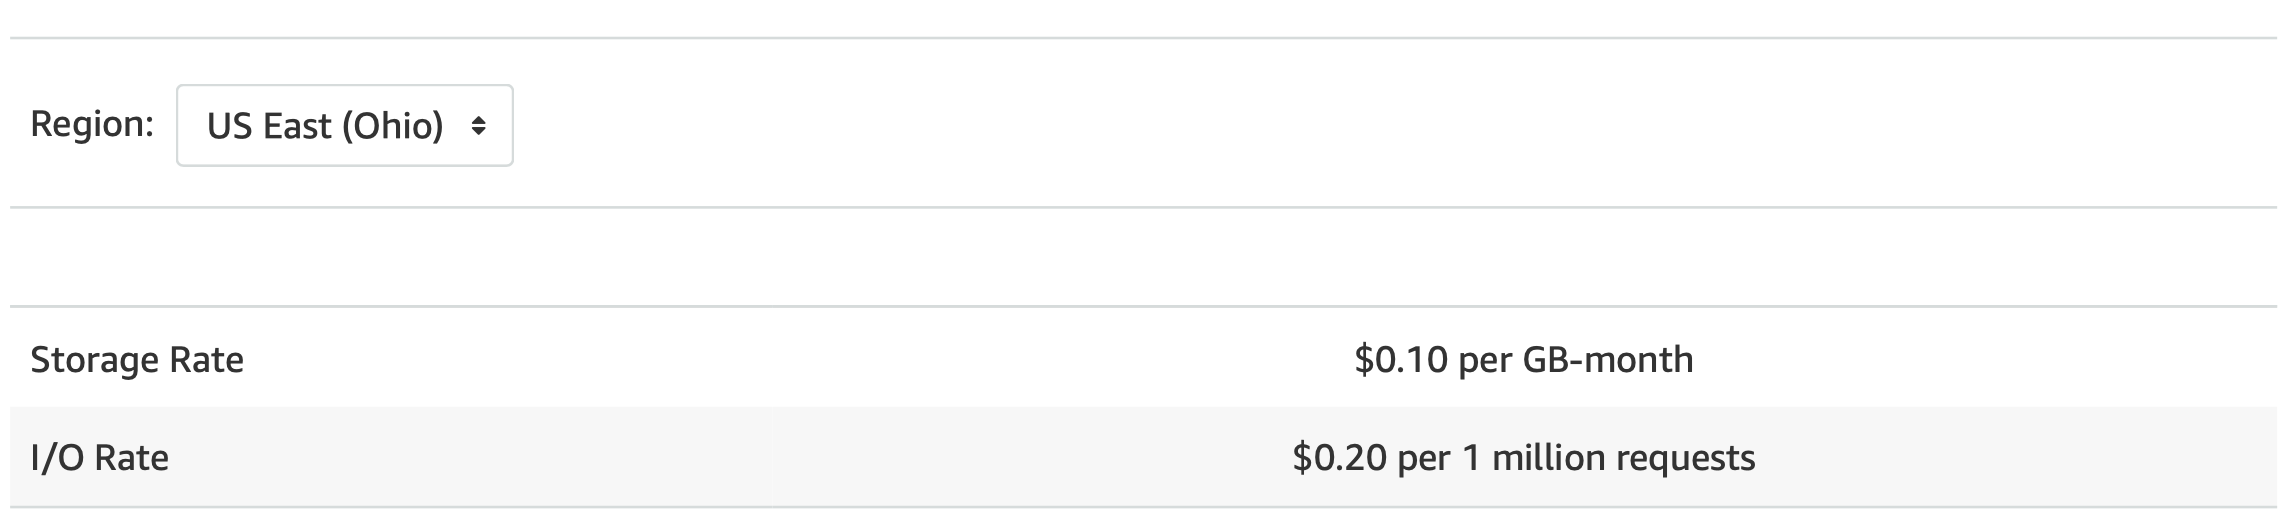
\includegraphics[width=12cm]{p1_3.png}
\end{center}
The cost of database for one month is $0.1 \times 1263.5 + 0.2 \times 47.27$ = $135.8$ USD per month. Also, to maintain database instance, a monthly cost of $6.96 \times 730$ = $5,080.8$ USD is needed.
\\
\\
The license plate image recognition should handle $47.27$ million requests, according to the pricing information\footnote{https://aws.amazon.com/rekognition/pricing/?nc1=h\_ls}, 
\begin{center}
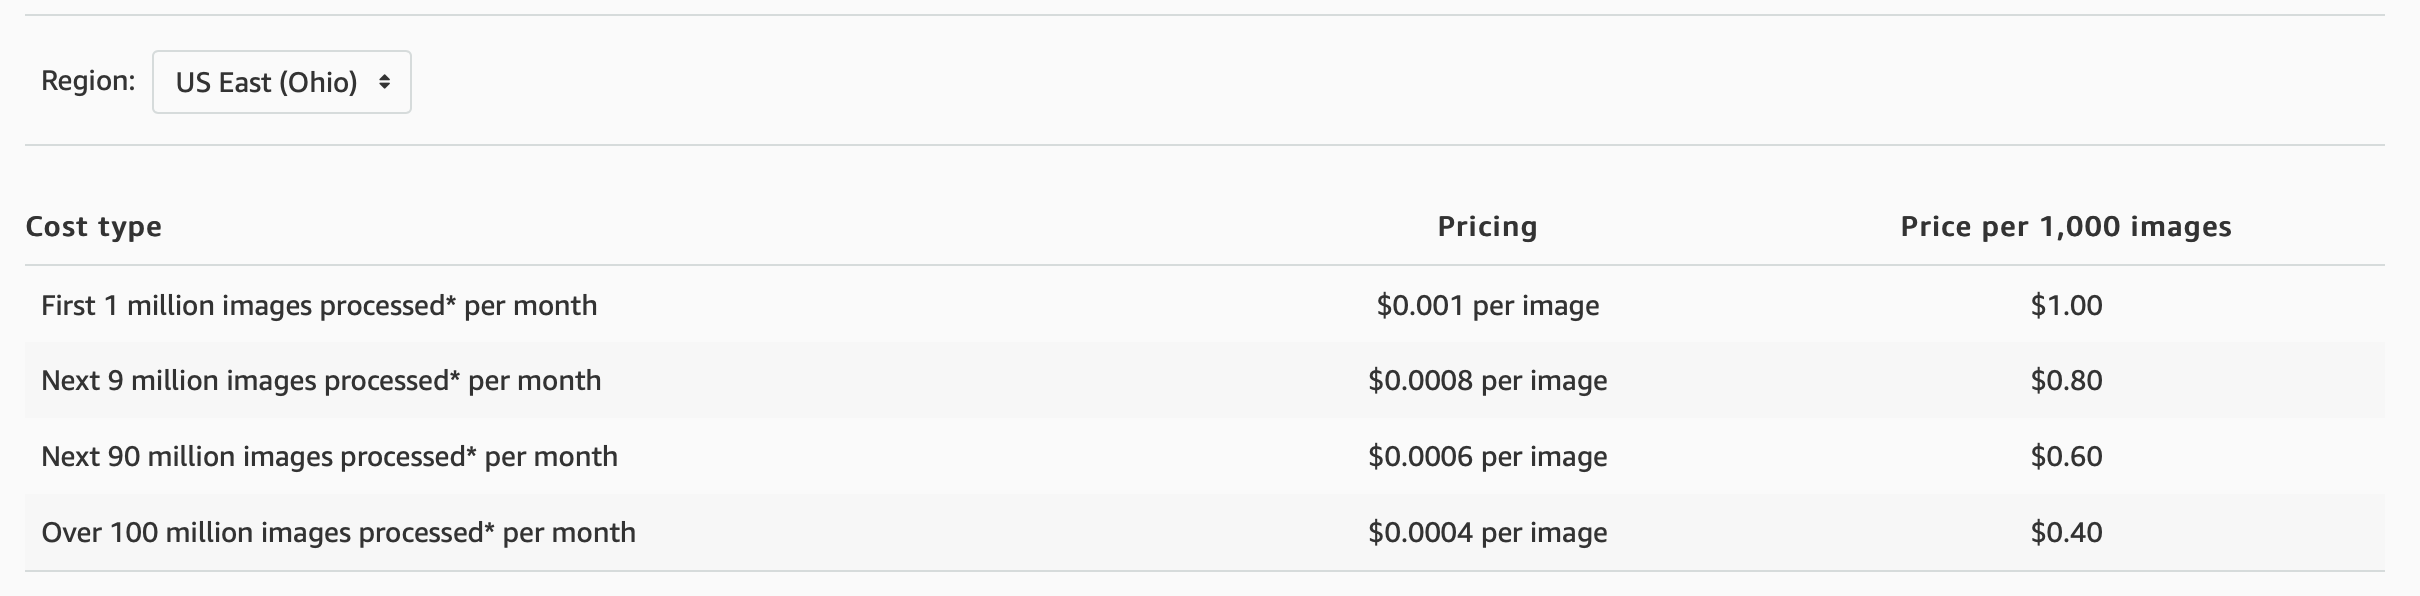
\includegraphics[width=15cm]{p1_33.png}
\end{center}
The cost of license plate image recognition for one month is $1,000 + 7,200 + 22,362$ = $30,562$ USD.
\\
\\
So the total monthly cost is $135.8 + 5,080.8 + 30,562$ = $35,778.6$ USD.
\end{solution}
% ---------------------------------------------------------
\HomeworkHeader{3}{2}	% homework number, problem number
\setcounter{page}{4}
\begin{solution}
(1) The matrix of cluster indices (shape: $6$×$6$) and the vector of
centroids (shape: $4$×$1$) are:
\begin{center}
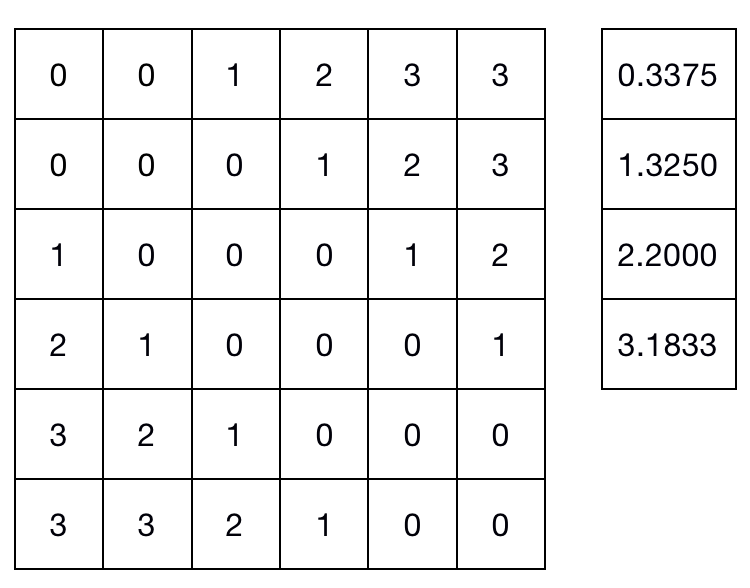
\includegraphics[width=10cm]{2_1.png}
\end{center}
where $0$ indicates $Group_0$, $1$ indicates $Group_1$, $2$ indicates $Group_2$, and $3$ indicates $Group_3$.\\
\\
The centroid of $Group_0$ is $0.3375$, the centroid of $Group_1$ is $1.3250$, the centroid of $Group_2$ is $2.200$, the centroid of $Group_3$ is $3.1833$.
\\
\\
(2) $2$ bits are required to encode $0, 1, 2, 3$, so there are $2 \times 36 = 72$ bits for the matrix of cluster indices; $32 \times 4 = 128$ bits for the vector of centroids. There are totally $72 + 128 = 200$ bits after weight quantization. Before weight quantization, there are $32 \times 36 = 1,152$ bits to encode weights, so the compression ratio = $\frac{\text{Uncompressed Size}}{\text{Compressed Size}}$ = $\frac{1,152}{200} = 5.76$. 
\\
\\
\pagebreak \\
(3) Hoffman encoding works as follows: we first find the frequency of each centroid, and we repeatedly split the set of centroids into two subsets with almost the same frequencies, for each "left arm", assign "$0$", and for each "right arm", assign "$1$".
\begin{center}
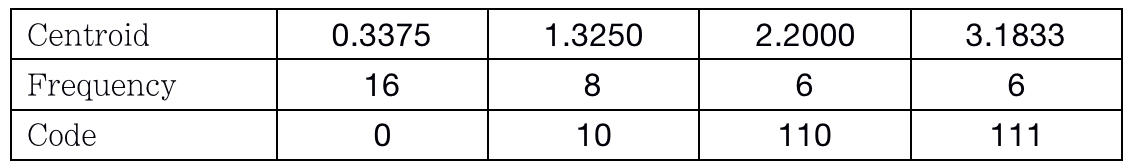
\includegraphics[width=10cm]{2_3_1.png}
\end{center}
\begin{center}
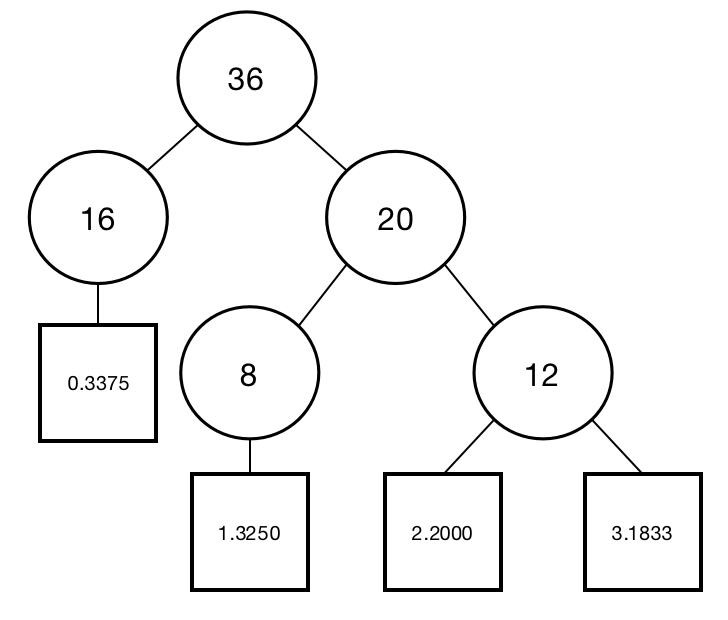
\includegraphics[width=6cm]{2_3_2.png}
\end{center}
Fill the encoded data into the $6 \times 6$ matrix,
\begin{center}
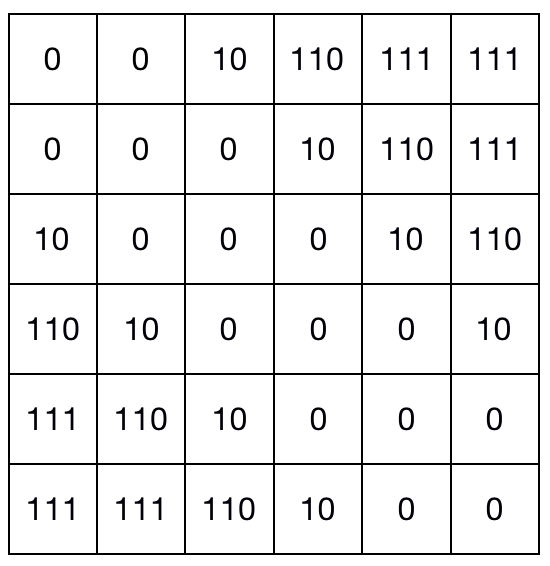
\includegraphics[width=8cm]{2_3_3.png}
\end{center}
There are $1 \times 16 + 2 \times 8 + 3 \times 6 + 3 \times 6 = 68$ bits for the matrix of cluster indices after Hoffman encoding, compared to $72$ bits before Hoffman encoding, we can save $4$ bits of memory.
\end{solution}
% ---------------------------------------------------------
\HomeworkHeader{3}{3}	% homework number, problem number
\setcounter{page}{6}
\begin{solution}
(1-a) RISC is the acronym for "Reduced Instruction Set Computer", is a type of microprocessor architecture that utilizes a small, highly-optimized set of instructions, rather than a larger and more specialized set of instructions.\footnote{https://cs.stanford.edu/people/eroberts/courses/soco/projects/risc/whatis/index.html}.
\\
\\
Therefore, the main characteristics of RISC ISA can be concluded as: (1) the set of instructions is small and highly-optimized, (2) instructions are executed with higher speed and shorter time, (3) RISC ISA allows freedom of using space on microprocessors because of its simplicity.
\\
\\
(1-b) Two main characteristics of the Power ISA: (1) Power ISA is a $64$-bit architecture with a $32$-bit subset, all code written by the $32$-bit subset could run on a $64$-bit machine, (2) Power ISA features a virtual address system which maps all addresses into a $52$-bit space, such that applications can share memory in a "flat" $32$-bit space, and all of the programs can have different blocks of $32$ bits each\footnote{https://en.wikipedia.org/wiki/IBM\_POWER\_instruction\_set\_architecture}.
\\
\\
What POWER systems are: Power Systems is a family of server computers from IBM that are based on its POWER processors. The aim of these accelerated computing servers is for modern analytics, high-performance computing HPC, and Artificial intelligence\footnote{https://en.wikipedia.org/wiki/IBM\_Power\_Systems}. 
\\
\\
(1-c) I will summarize two similarities and two differences, for similarities,
\begin{itemize}
\item All three architectures support byte addressing, whcih means they can access individual bytes of data rather than only larger units of data (called "word").
\item All three architectures support two's complement and floating point for standard arithmetic, logical, and shift operations.
\end{itemize}
for differences,
\begin{itemize}
\item Intel x86 is designed as CISC, while ARM and Power ISA are designed as RISC.
\item Intel x86 is little-endian, while most RISC architectures are originally big-endian, so as the Power ISA, but ARM is little-endian.
\end{itemize}
(2-a) CAPI (Coherent Accelerator Processor Interface) is a high-speed processor expansion bus standard, initially designed to be layered on top of PCI Express, for directly connecting CPUs to external accelerators like GPUs, ASICs, FPGAs or fast storage. It offers low latency, high speed, direct memory access connectivity between devices of different instruction set architectures\footnote{https://en.wikipedia.org/wiki/Coherent\_Accelerator\_Processor\_Interface}.
\\
\\
One significant problem that CAPI aims to solve is to enable computers to more easily and efficiently attach specialized accelerators, because in many applications, accelerators struggle with limitations of the interconnect's performance (bandwidth and latency) or with limitations due to the interconnect's architecture (such as lacking memory coherence)\footnote{https://en.wikipedia.org/wiki/Coherent\_Accelerator\_Processor\_Interface}.
\\
\\
(2-b) SNAP is the acronym for "Storage, Network, Analytics, Programming",  a framework that enables programmers and computer engineers to quickly create FPGA-based acceleration actions that work on server host data, as well as data from storage, flash, Ethernet, or other connected resources\footnote{https://github.com/open-power/snap}. 
\\
\\
The relationship between CAPI and SNAP is that SNAP framework uses CAPI infrastructure which provides the technology and ecosystem foundation to realize hardware acceleration.
\\
\\
(2-c) For i, 
\begin{itemize}
\item (1) HOST memory
\item (2) PSL
\item (3) AXI
\item (4) Hardware Action
\item (5) Device Memory
\end{itemize}
For ii, (1) The host issues an NVMe read request to the FPGA through MMIO registers; (2) FPGA reads data from NVMe SSD through AXI and writes data to device memory; (3) The host allocates device memory, calls FPGA to start computation, and waits for the result to be stored in device memory; (4) FPGA exectute computation, after completion, it notifies the host that the task is finished; (5) The host receives the information and deallocates FPGA resources. 
\end{solution}
% ---------------------------------------------------------
\HomeworkHeader{3}{4}	% homework number, problem number
\setcounter{page}{8}
\begin{solution}
(1-a) First compute the mean memory access latency by the following formula:
\\
\\
mean memory access latency = ($1$ $-$ miss rate) × access latency of current level
+ miss rate × mean access latency of next level,
\\
\\
mean memory access latency = ($1$ $-$ $10\%$) × $5$ + $10\%$ × mean access latency of $L_2$,
\\
\\
replace mean access latency of $L_2$ by ($1$ $-$ $5\%$) × $15$ + $5\%$ × mean access latency of $L_1$,
\\
\\
replace mean access latency of $L_1$ by ($1$ $-$ $2\%$) × $45$ + $2\%$ × $80$ = $45.7$ns,
\\
\\
we have mean memory access latency = $6.1535$ns.
\\
\\
Then, the total memory access time is given by the following formula:
\\
\\
total memory access time = mean latency × total number of accesses
+compulsory cache misses latency = $6.1535$ × $10^9$ + $80$ × $10^6$ = $6.2335$s.
\\
\\
(1-b) Similarly, by the same procedure, first compute the mean memory access energy by the following formula:
\\
\\
mean memory access energy = ($1$ $-$ miss rate) × access energy of current level
+ miss rate × mean access energy of next level,
\\
\\
mean memory access energy = ($1$ $-$ $10\%$) × $15$ + $10\%$ × mean access energy of $L_2$,
\\
\\
replace mean access energy of $L_2$ by ($1$ $-$ $5\%$) × $26$ + $5\%$ × mean access energy of $L_1$,
\\
\\
replace mean access energy of $L_1$ by ($1$ $-$ $2\%$) × $47$ + $2\%$ × $2560$ = $97.26$pJ,
\\
\\
we have mean memory access energy = $16.4563$pJ.
\\
\\
Then, the total memory access energy is given by the following formula:
\\
\\
total memory access energy = mean energy × total number of accesses
+compulsory cache misses energy = $16.4563$ × $10^9$ + $2560$ × $10^6$ = $1.90\times10^{10}$pJ.
\\
\\
(1-c) We have the following formula:
\\
\\
the percentage of total energy consumed by computation = $\frac{\text{total energy consumed by computation}}{\text{total energy consumed by computation + total memory access energy}} \times 100\%$ = $\frac{18}{18 + 16.4563 \times 3} \times 100\% = 26.72\%$.
\\
\\
(2) First compute the mean memory access latency by the following formula:
\\
\\
mean memory access latency = ($1$ $-$ miss rate) × access latency of current level
+ miss rate × mean access latency of next level,
\\
\\
mean memory access latency = ($1$ $-$ $10\%$) × $5$ + $10\%$ × mean access latency of $L_2$,
\\
\\
replace mean access latency of $L_2$ by ($1$ $-$ $5\%$) × $15$ + $5\%$ × mean access latency of $L_1$,
\\
\\
replace mean access latency of $L_1$ by ($1$ $-$ $2\%$) × $45$ + $2\%$ × $40$ = $44.9$ns,
\\
\\
we have mean memory access latency = $6.1495$ns.
\\
\\
Then, the total memory access time is given by the following formula:
\\
\\
total memory access time = mean latency × total number of accesses
+compulsory cache misses latency = $6.1495$ × $10^9$ + $40$ × $10^6$ = $6.1895$s.
\\
\\
Similarly, by the same procedure, first compute the mean memory access energy by the following formula:
\\
\\
mean memory access energy = ($1$ $-$ miss rate) × access energy of current level
+ miss rate × mean access energy of next level,
\\
\\
mean memory access energy = ($1$ $-$ $10\%$) × $15$ + $10\%$ × mean access energy of $L_2$,
\\
\\
replace mean access energy of $L_2$ by ($1$ $-$ $5\%$) × $26$ + $5\%$ × mean access energy of $L_1$,
\\
\\
replace mean access energy of $L_1$ by ($1$ $-$ $2\%$) × $47$ + $2\%$ × $1280$ = $71.66$pJ,
\\
\\
we have mean memory access energy = $16.3283$pJ.
\\
\\
Then, the total memory access energy is given by the following formula:
\\
\\
total memory access energy = mean energy × total number of accesses
+compulsory cache misses energy = $16.3283$ × $10^9$ + $1280$ × $10^6$ = $1.76\times10^{10}$pJ.
\\
\\
(3) We can see that by implementing NMA, both total memory access time and energy can be reduced, because it brings computation closer to memory, which reduce both latency and energy spent on data transmission between CPU and memory.
\end{solution}
% ---------------------------------------------------------
\HomeworkHeader{3}{5}	% homework number, problem number
\setcounter{page}{10}
\begin{solution}
(1) From HW$2$, we know \textbf{\# of operations} = \# of input channels $\times$ \# of output channels $\times$ output width $\times$ output height $\times$ filter size $\times 2$ = $d_i \times d_j \times h_i \times w_i \times k \times k \times 2$.
\\
\\
(2) For only depthwise convolution, \textbf{\# of operations} = \# of input channels $\times$ output width $\times$ output height $\times$ filter size $\times 2$ = $d_i \times h_i \times w_i \times k \times k \times 2$. Because there is a one-to-one correspondence between input features and channels.
\\
\\
(3) For only pointwise convolution, \textbf{\# of operations} = \# of input channels $\times$ \# of output channels $\times$ output width $\times$ output height $\times 2$ = $d_i \times d_j \times h_i \times w_i \times 2$. Because pointwise is responsible for building new features through computing linear combinations of the input channels\footnote{Mark Sandler, et al. "MobileNetV2: Inverted Residuals and Linear Bottlenecks". \textit{The IEEE Conference on Computer Vision and Pattern Recognition (CVPR)}, 2018, pp. 4510-4520}.
\\
\\
(4) So by combination of depthwise convolution and pointwise convolution, \textbf{\# of operations} = $d_i \times h_i \times w_i \times k \times k \times 2$ + $d_i \times d_j \times h_i \times w_i \times 2$.
\\
\\
\textbf{The ratio of operation reduction} = $1 - \frac{d_i \times h_i \times w_i \times k \times k \times 2 + d_i \times d_j \times h_i \times w_i \times 2}{d_i \times d_j \times h_i \times w_i \times k \times k \times 2}$ = $1 - \frac{1}{d_j} - \frac{1}{k^2}$
\\
\\
It can save operations because as a drop-in replacement for standard convolution, depthwise separable convolution replaces a full convolutional operator with a factorized version that splits convolution into two stages\footnote{Mark Sandler, et al. "MobileNetV2: Inverted Residuals and Linear Bottlenecks"}, namely, the depthwise convolution and pointwise convolution.
The original kernels are divided into two smaller kernels and the original convolution is divided into two different stages, and the number of operations is reduced because of the one-to-one correspondence between input features and channels (this mainly reduces the number of operations for depthwise convolution) and smaller kernel sizes (this mainly reduces the number of operations for pointwise convolution).
\end{solution}
% ---------------------------------------------------------

\end{document}
